\chapter{جستجوی کامل}

\key{جستجوی کامل}
روشی کلی برای حل تقریباً هر مسئلهٔ الگوریتمی است.
ایدهٔ اصلی، تولید تمام پاسخ‌های ممکن برای مسئله با استفاده از روش نیروی بی‌رحم (brute force)،
و سپس انتخاب بهترین پاسخ یا شمارش تعداد پاسخ‌ها، بسته به صورت مسئله است.

اگر زمان کافی برای بررسی همهٔ پاسخ‌ها وجود داشته باشد، جستجوی کامل تکنیک مناسبی است؛
زیرا پیاده‌سازی این جستجو معمولاً آسان است
و همیشه پاسخ درست می‌دهد.
اگر جستجوی کامل بسیار کُند باشد،
تکنیک‌های دیگر نظیر الگوریتم‌های حریصانه یا
برنامه‌نویسی پویا ممکن است مورد نیاز باشند.

\section{تولید زیرمجموعه‌ها}

\index{زیرمجموعه}

ابتدا مسئلهٔ تولید
تمام زیرمجموعه‌های یک مجموعهٔ $n$ عضوی را بررسی می‌کنیم.
به عنوان مثال، زیرمجموعه‌های $\{0,1,2\}$ عبارتند از:
$\emptyset$، $\{0\}$، $\{1\}$، $\{2\}$، $\{0,1\}$،
$\{0,2\}$، $\{1,2\}$ و $\{0,1,2\}$.
دو روش رایج برای تولید زیرمجموعه‌ها وجود دارد:
می‌توان از یک جستجوی بازگشتی استفاده کرد
یا از نمایش بیتی اعداد صحیح بهره برد.

\subsubsection{روش ۱}

یک روش هوشمندانه برای پیمایش تمام زیرمجموعه‌های
یک مجموعه، استفاده از بازگشت است.
تابع زیر با نام \texttt{search}
زیرمجموعه‌های مجموعهٔ
$\{0,1,\ldots,n-1\}$ را تولید می‌کند.
این تابع یک بردار به نام \texttt{subset} را نگه می‌دارد
که شامل عناصر هر زیرمجموعه خواهد بود.
جستجو زمانی آغاز می‌شود که تابع
با پارامتر 0 فراخوانی شود.

\begin{lstlisting}
void search(int k) {
    if (k == n) {
        // process subset
    } else {
        search(k+1);
        subset.push_back(k);
        search(k+1);
        subset.pop_back();
    }
}
\end{lstlisting}

هنگامی که تابع \texttt{search}
با پارامتر $k$ فراخوانی می‌شود،
تصمیم می‌گیرد که آیا عنصر
$k$ را در زیرمجموعه قرار دهد یا خیر،
و در هر دو حالت،
سپس خود را با پارامتر $k+1$ فراخوانی می‌کند.
با این حال، اگر $k=n$ باشد، تابع متوجه می‌شود که
همهٔ عناصر پردازش شده‌اند
و یک زیرمجموعه تولید شده است.

درخت زیر فراخوانی‌های تابع را در حالتی که $n=3$ است نشان می‌دهد.
ما همواره می‌توانیم شاخهٔ چپ
(عنصر $k$ در زیرمجموعه قرار نمی‌گیرد) یا شاخهٔ راست
(عنصر $k$ در زیرمجموعه قرار می‌گیرد) را انتخاب کنیم.

\begin{center}
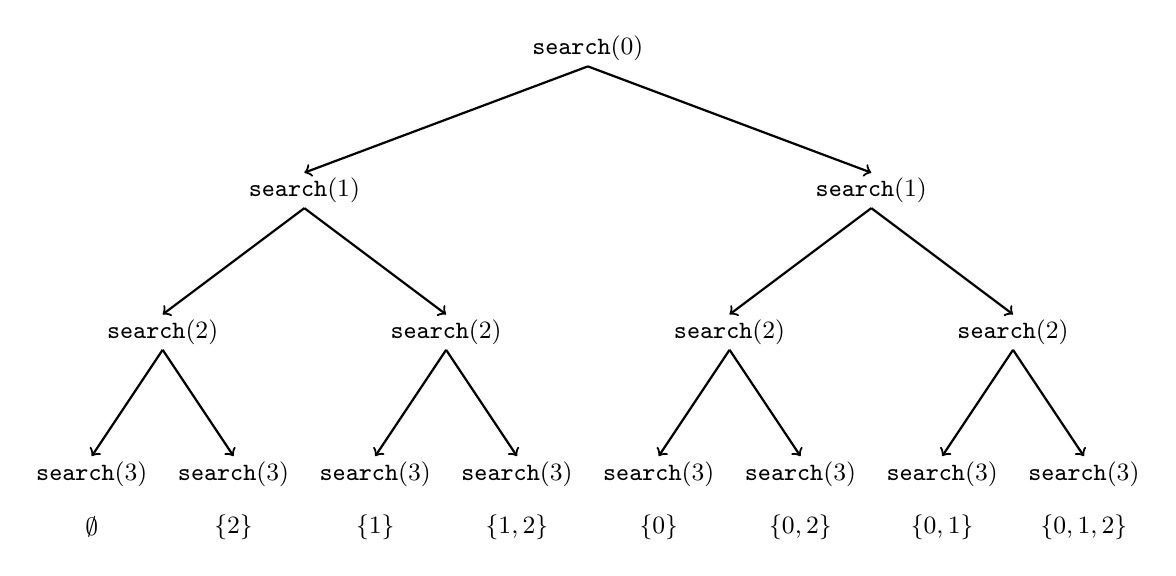
\begin{tikzpicture}[scale=.45]
  \begin{scope}
    \small
    \node at (0,0) {$\texttt{search}(0)$};

    \node at (-8,-4) {$\texttt{search}(1)$};
    \node at (8,-4) {$\texttt{search}(1)$};

    \path[draw,thick,->] (0,0-0.5) -- (-8,-4+0.5);
    \path[draw,thick,->] (0,0-0.5) -- (8,-4+0.5);

    \node at (-12,-8) {$\texttt{search}(2)$};
    \node at (-4,-8) {$\texttt{search}(2)$};
    \node at (4,-8) {$\texttt{search}(2)$};
    \node at (12,-8) {$\texttt{search}(2)$};

    \path[draw,thick,->] (-8,-4-0.5) -- (-12,-8+0.5);
    \path[draw,thick,->] (-8,-4-0.5) -- (-4,-8+0.5);
    \path[draw,thick,->] (8,-4-0.5) -- (4,-8+0.5);
    \path[draw,thick,->] (8,-4-0.5) -- (12,-8+0.5);

    \node at (-14,-12) {$\texttt{search}(3)$};
    \node at (-10,-12) {$\texttt{search}(3)$};
    \node at (-6,-12) {$\texttt{search}(3)$};
    \node at (-2,-12) {$\texttt{search}(3)$};
    \node at (2,-12) {$\texttt{search}(3)$};
    \node at (6,-12) {$\texttt{search}(3)$};
    \node at (10,-12) {$\texttt{search}(3)$};
    \node at (14,-12) {$\texttt{search}(3)$};

    \node at (-14,-13.5) {$\emptyset$};
    \node at (-10,-13.5) {$\{2\}$};
    \node at (-6,-13.5) {$\{1\}$};
    \node at (-2,-13.5) {$\{1,2\}$};
    \node at (2,-13.5) {$\{0\}$};
    \node at (6,-13.5) {$\{0,2\}$};
    \node at (10,-13.5) {$\{0,1\}$};
    \node at (14,-13.5) {$\{0,1,2\}$};


    \path[draw,thick,->] (-12,-8-0.5) -- (-14,-12+0.5);
    \path[draw,thick,->] (-12,-8-0.5) -- (-10,-12+0.5);
    \path[draw,thick,->] (-4,-8-0.5) -- (-6,-12+0.5);
    \path[draw,thick,->] (-4,-8-0.5) -- (-2,-12+0.5);
    \path[draw,thick,->] (4,-8-0.5) -- (2,-12+0.5);
    \path[draw,thick,->] (4,-8-0.5) -- (6,-12+0.5);
    \path[draw,thick,->] (12,-8-0.5) -- (10,-12+0.5);
    \path[draw,thick,->] (12,-8-0.5) -- (14,-12+0.5);
\end{scope}
\end{tikzpicture}
\end{center}

\subsubsection{روش ۲}

روش دیگر تولید زیرمجموعه‌ها بر پایه نمایش بیتی اعداد صحیح است.
هر زیرمجموعه از یک مجموعه $n$ عضوی را می‌توان به شکل دنباله‌ای از $n$ بیت نشان داد،
که متناظر با یک عدد صحیح بین $0 \ldots 2^n-1$ است.
یک‌ها در دنباله بیتی مشخص می‌کنند کدام عضوها در زیرمجموعه حضور دارند.

قرارداد معمول این است که
بیت آخر متناظر با عضو 0،
بیت ماقبل آخر متناظر با عضو 1،
و به همین ترتیب باشد.
برای نمونه، نمایش بیتی عدد 25
برابر 11001 است که با زیرمجموعه $\{0,3,4\}$ تناظر دارد.

کد زیر تمام زیرمجموعه‌های یک مجموعه $n$ عضوی را پیمایش می‌کند:

\begin{lstlisting}
for (int b = 0; b < (1<<n); b++) {
    // پردازش زیرمجموعه
}
\end{lstlisting}

کد زیر نشان می‌دهد چگونه می‌توان اعضای زیرمجموعه متناظر با یک دنباله بیتی را به دست آورد.
هنگام پردازش هر زیرمجموعه،
کد یک بردار شامل اعضای موجود در زیرمجموعه می‌سازد.

\begin{lstlisting}
for (int b = 0; b < (1<<n); b++) {
    vector<int> subset;
    for (int i = 0; i < n; i++) {
        if (b&(1<<i)) subset.push_back(i);
    }
}
\end{lstlisting}

\section{تولید جایگشت‌ها}

\index{permutation}

در ادامه مسئله تولید تمام جایگشت‌های یک مجموعه $n$ عضوی بررسی می‌شود.
برای نمونه، جایگشت‌های $\{0,1,2\}$ عبارتند از
$(0,1,2)$، $(0,2,1)$، $(1,0,2)$، $(1,2,0)$،
$(2,0,1)$ و $(2,1,0)$.
اینجا نیز دو رویکرد وجود دارد:
می‌توان از بازگشت بهره برد یا جایگشت‌ها را به روش تکراری پیمایش کرد.

\subsubsection{روش ۱}

همانند زیرمجموعه‌ها، جایگشت‌ها را نیز می‌توان با بازگشت تولید کرد.
تابع \texttt{search} زیر
جایگشت‌های مجموعه $\{0,1,\ldots,n-1\}$ را پیمایش می‌کند.
تابع بردار \texttt{permutation} حاوی جایگشت را می‌سازد،
و جستجو با فراخوانی تابع بدون آرگومان آغاز می‌شود.

\begin{lstlisting}
void search() {
    if (permutation.size() == n) {
        // process permutation
    } else {
        for (int i = 0; i < n; i++) {
            if (chosen[i]) continue;
            chosen[i] = true;
            permutation.push_back(i);
            search();
            chosen[i] = false;
            permutation.pop_back();
        }
    }
}
\end{lstlisting}

هر فراخوانی تابع یک عنصر جدید به \texttt{permutation} اضافه می‌کند.
آرایه \texttt{chosen} مشخص می‌کند کدام عناصر قبلاً در جایگشت قرار گرفته‌اند.
اگر اندازه \texttt{permutation} برابر با اندازه مجموعه شود، یک جایگشت تولید شده است.

\subsubsection{روش ۲}

\index{next\_permutation@\texttt{next\_permutation}}

روش دیگر برای تولید جایگشت‌ها، شروع با جایگشت $\{0,1,\ldots,n-1\}$ و استفاده متوالی از تابعی است که جایگشت بعدی را به ترتیب صعودی می‌سازد.
کتابخانه استاندارد C++ شامل تابع \texttt{next\_permutation} است که می‌تواند برای این کار استفاده شود:

\begin{lstlisting}
vector<int> permutation;
for (int i = 0; i < n; i++) {
    permutation.push_back(i);
}
do {
    // process permutation
} while (next_permutation(permutation.begin(),permutation.end()));
\end{lstlisting}

\section{عقب‌گرد}

\index{backtracking@عقب‌گرد}

یک الگوریتم \key{عقب‌گرد} (backtracking) با یک جواب خالی شروع می‌شود و جواب را گام به گام گسترش می‌دهد.
جستجو به صورت بازگشتی تمام روش‌های مختلف ساخت یک جواب را بررسی می‌کند.

\index{queen problem@مسئله وزیرها}

به عنوان مثال، مسئله محاسبه تعداد روش‌های قرار دادن $n$ وزیر در یک صفحه شطرنج $n \times n$ را در نظر بگیرید، به طوری که هیچ دو وزیری یکدیگر را تهدید نکنند.
برای نمونه، زمانی که $n=4$ است، دو جواب ممکن وجود دارد:

\begin{center}
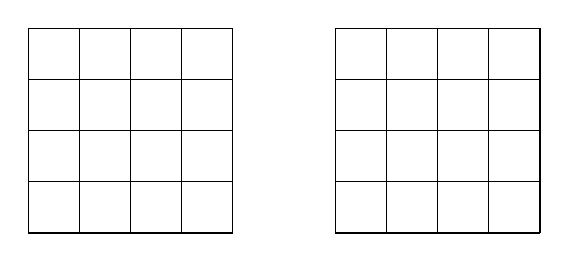
\begin{tikzpicture}[scale=.65]
  \begin{scope}
    \draw (0, 0) grid (4, 4);
    \node at (1.5,3.5) {\symqueen};
    \node at (3.5,2.5) {\symqueen};
    \node at (0.5,1.5) {\symqueen};
    \node at (2.5,0.5) {\symqueen};

    \draw (6, 0) grid (10, 4);
    \node at (6+2.5,3.5) {\symqueen};
    \node at (6+0.5,2.5) {\symqueen};
    \node at (6+3.5,1.5) {\symqueen};
    \node at (6+1.5,0.5) {\symqueen};

  \end{scope}
\end{tikzpicture}
\end{center}

این مسئله را می‌توان با عقب‌گرد و قرار دادن سطر به سطر وزیرها در صفحه حل کرد.
به طور دقیق‌تر، دقیقاً یک وزیر در هر سطر قرار می‌گیرد، به طوری که هیچ وزیری به وزیرهای قرار داده شده قبلی حمله نکند.
هنگامی که همه $n$ وزیر در صفحه قرار گرفتند، یک جواب پیدا شده است.

برای نمونه، وقتی $n=4$ است، برخی از جواب‌های جزئی تولید شده توسط الگوریتم عقب‌گرد به صورت زیر هستند:

\begin{center}
\begin{tikzpicture}[scale=.55]
  \begin{scope}
    \draw (0, 0) grid (4, 4);

    \draw (-9, -6) grid (-5, -2);
    \draw (-3, -6) grid (1, -2);
    \draw (3, -6) grid (7, -2);
    \draw (9, -6) grid (13, -2);

    \node at (-9+0.5,-3+0.5) {\symqueen};
    \node at (-3+1+0.5,-3+0.5) {\symqueen};
    \node at (3+2+0.5,-3+0.5) {\symqueen};
    \node at (9+3+0.5,-3+0.5) {\symqueen};

    \draw (2,0) -- (-7,-2);
    \draw (2,0) -- (-1,-2);
    \draw (2,0) -- (5,-2);
    \draw (2,0) -- (11,-2);

    \draw (-11, -12) grid (-7, -8);
    \draw (-6, -12) grid (-2, -8);
    \draw (-1, -12) grid (3, -8);
    \draw (4, -12) grid (8, -8);
    \draw[white] (11, -12) grid (15, -8);
    \node at (-11+1+0.5,-9+0.5) {\symqueen};
    \node at (-6+1+0.5,-9+0.5) {\symqueen};
    \node at (-1+1+0.5,-9+0.5) {\symqueen};
    \node at (4+1+0.5,-9+0.5) {\symqueen};
    \node at (-11+0+0.5,-10+0.5) {\symqueen};
    \node at (-6+1+0.5,-10+0.5) {\symqueen};
    \node at (-1+2+0.5,-10+0.5) {\symqueen};
    \node at (4+3+0.5,-10+0.5) {\symqueen};

    \draw (-1,-6) -- (-9,-8);
    \draw (-1,-6) -- (-4,-8);
    \draw (-1,-6) -- (1,-8);
    \draw (-1,-6) -- (6,-8);

    \node at (-9,-13) {غیرمجاز};
    \node at (-4,-13) {غیرمجاز};
    \node at (1,-13) {غیرمجاز};
    \node at (6,-13) {معتبر};

  \end{scope}
\end{tikzpicture}
\end{center}

در پایین‌ترین سطح، سه پیکربندی اول
غیرمجاز هستند، زیرا وزیرها به یکدیگر حمله می‌کنند.
با این حال، پیکربندی چهارم معتبر است
و می‌توان آن را با قرار دادن دو وزیر دیگر در صفحه
به یک پاسخ کامل گسترش داد.
تنها یک راه برای قرار دادن دو وزیر باقی‌مانده وجود دارد.

\begin{samepage}
الگوریتم را می‌توان به صورت زیر پیاده‌سازی کرد:
\begin{lstlisting}
void search(int y) {
    if (y == n) {
        count++;
        return;
    }
    for (int x = 0; x < n; x++) {
        if (column[x] || diag1[x+y] || diag2[x-y+n-1]) continue;
        column[x] = diag1[x+y] = diag2[x-y+n-1] = 1;
        search(y+1);
        column[x] = diag1[x+y] = diag2[x-y+n-1] = 0;
    }
}
\end{lstlisting}
\end{samepage}
جستجو با فراخوانی \texttt{search(0)} آغاز می‌شود.
اندازه صفحه $n \times n$ است
و کد تعداد پاسخ‌ها را در متغیر \texttt{count} محاسبه می‌کند.

کد فرض می‌کند که سطرها و ستون‌های
صفحه از 0 تا $n-1$ شماره‌گذاری شده‌اند.
هنگامی که تابع \texttt{search} با آرگومان $y$ فراخوانی می‌شود،
وزیری را در سطر $y$ قرار می‌دهد
و سپس خود را با آرگومان $y+1$ فراخوانی می‌کند.
سپس، اگر $y=n$ باشد، یک پاسخ یافت شده است
و متغیر \texttt{count} یک واحد افزایش می‌یابد.

آرایه \texttt{column} ستون‌هایی را که شامل وزیر هستند پیگیری می‌کند،
و آرایه‌های \texttt{diag1} و \texttt{diag2}
قطرها را دنبال می‌کنند.
اضافه کردن وزیری دیگر به ستون یا قطری که از قبل شامل وزیر است،
مجاز نیست.
برای مثال، ستون‌ها و قطرهای
صفحه $4 \times 4$ به صورت زیر شماره‌گذاری می‌شوند:

\begin{center}
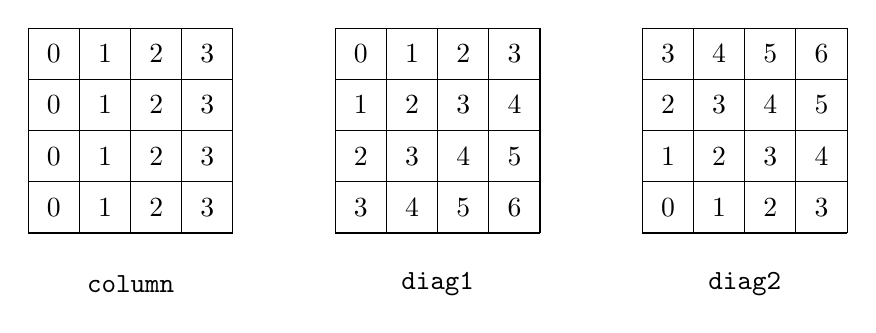
\begin{tikzpicture}[scale=.65]
  \begin{scope}
    \draw (0-6, 0) grid (4-6, 4);
    \node at (-6+0.5,3.5) {$0$};
    \node at (-6+1.5,3.5) {$1$};
    \node at (-6+2.5,3.5) {$2$};
    \node at (-6+3.5,3.5) {$3$};
    \node at (-6+0.5,2.5) {$0$};
    \node at (-6+1.5,2.5) {$1$};
    \node at (-6+2.5,2.5) {$2$};
    \node at (-6+3.5,2.5) {$3$};
    \node at (-6+0.5,1.5) {$0$};
    \node at (-6+1.5,1.5) {$1$};
    \node at (-6+2.5,1.5) {$2$};
    \node at (-6+3.5,1.5) {$3$};
    \node at (-6+0.5,0.5) {$0$};
    \node at (-6+1.5,0.5) {$1$};
    \node at (-6+2.5,0.5) {$2$};
    \node at (-6+3.5,0.5) {$3$};

    \draw (0, 0) grid (4, 4);
    \node at (0.5,3.5) {$0$};
    \node at (1.5,3.5) {$1$};
    \node at (2.5,3.5) {$2$};
    \node at (3.5,3.5) {$3$};
    \node at (0.5,2.5) {$1$};
    \node at (1.5,2.5) {$2$};
    \node at (2.5,2.5) {$3$};
    \node at (3.5,2.5) {$4$};
    \node at (0.5,1.5) {$2$};
    \node at (1.5,1.5) {$3$};
    \node at (2.5,1.5) {$4$};
    \node at (3.5,1.5) {$5$};
    \node at (0.5,0.5) {$3$};
    \node at (1.5,0.5) {$4$};
    \node at (2.5,0.5) {$5$};
    \node at (3.5,0.5) {$6$};

    \draw (6, 0) grid (10, 4);
    \node at (6.5,3.5) {$3$};
    \node at (7.5,3.5) {$4$};
    \node at (8.5,3.5) {$5$};
    \node at (9.5,3.5) {$6$};
    \node at (6.5,2.5) {$2$};
    \node at (7.5,2.5) {$3$};
    \node at (8.5,2.5) {$4$};
    \node at (9.5,2.5) {$5$};
    \node at (6.5,1.5) {$1$};
    \node at (7.5,1.5) {$2$};
    \node at (8.5,1.5) {$3$};
    \node at (9.5,1.5) {$4$};
    \node at (6.5,0.5) {$0$};
    \node at (7.5,0.5) {$1$};
    \node at (8.5,0.5) {$2$};
    \node at (9.5,0.5) {$3$};

    \node at (-4,-1) {\texttt{column}};
    \node at (2,-1) {\texttt{diag1}};
    \node at (8,-1) {\texttt{diag2}};

  \end{scope}
\end{tikzpicture}
\end{center}

فرض کنید $q(n)$ نشان‌دهنده تعداد روش‌های
قرار دادن $n$ وزیر در یک صفحه شطرنج $n \times n$ باشد.
الگوریتم عقب‌گرد بالا
نشان می‌دهد که به عنوان مثال، $q(8)=92$ است.
با افزایش $n$، جستجو به سرعت کند می‌شود،
زیرا تعداد جواب‌ها
به صورت نمایی رشد می‌کند.
برای نمونه، محاسبه $q(16)=14772512$
با الگوریتم بالا روی یک رایانه امروزی
حدود یک دقیقه زمان می‌برد\footnote{روش کارآمد شناخته‌شده‌ای برای
محاسبه مقادیر بزرگتر $q(n)$ وجود ندارد. رکورد فعلی
$q(27)=234907967154122528$ است که در سال ۲۰۱۶ محاسبه شد \cite{q27}.}.

\section{هرس کردن جستجو}

اغلب می‌توان عقب‌گرد را
با هرس کردن درخت جستجو بهینه‌سازی کرد.
ایده اصلی، افزودن «هوشمندی» به الگوریتم است
تا در سریع‌ترین زمان ممکن تشخیص دهد
که آیا یک جواب جزئی قابلیت تبدیل
به یک جواب کامل را ندارد یا خیر.
چنین بهینه‌سازی‌هایی می‌توانند تأثیر
چشمگیری بر کارایی جستجو داشته باشند.

مسئله شمارش تعداد مسیرها
در یک شبکه $n \times n$ از گوشه بالا-چپ
به گوشه پایین-راست را در نظر بگیرید، به طوری که
مسیر دقیقاً یک بار از هر خانه عبور کند.
به عنوان مثال، در یک شبکه $7 \times 7$،
تعداد ۱۱۱۷۱۲ مسیر از این نوع وجود دارد.
یکی از این مسیرها به صورت زیر است:

\begin{center}
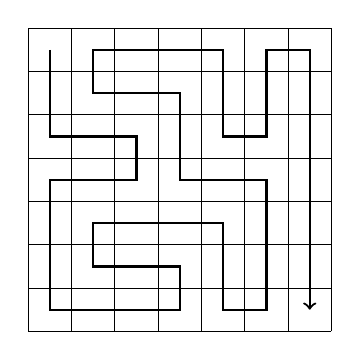
\begin{tikzpicture}[scale=.55]
  \begin{scope}
    \draw (0, 0) grid (7, 7);
    \draw[thick,->] (0.5,6.5) -- (0.5,4.5) -- (2.5,4.5) --
          (2.5,3.5) -- (0.5,3.5) -- (0.5,0.5) --
          (3.5,0.5) -- (3.5,1.5) -- (1.5,1.5) --
          (1.5,2.5) -- (4.5,2.5) -- (4.5,0.5) --
          (5.5,0.5) -- (5.5,3.5) -- (3.5,3.5) --
          (3.5,5.5) -- (1.5,5.5) -- (1.5,6.5) --
          (4.5,6.5) -- (4.5,4.5) -- (5.5,4.5) --
          (5.5,6.5) -- (6.5,6.5) -- (6.5,0.5);
  \end{scope}
\end{tikzpicture}
\end{center}

تمرکز ما روی حالت $7 \times 7$ است، زیرا سطح دشواری آن متناسب با نیاز ماست. کار را با الگوریتم عقب‌گرد ساده آغاز می‌کنیم و سپس با مشاهداتی درباره نحوه هرس جستجو، آن را گام به گام بهینه‌سازی می‌کنیم. پس از هر بهینه‌سازی، زمان اجرای الگوریتم و تعداد فراخوانی‌های بازگشتی را اندازه می‌گیریم تا تأثیر هر بهینه‌سازی بر کارایی جستجو مشخص شود.

\subsubsection{الگوریتم پایه}

نسخه نخست الگوریتم فاقد هرگونه بهینه‌سازی است. صرفاً با عقب‌گرد، تمام مسیرهای ممکن از گوشه بالا-چپ به گوشه پایین-راست تولید و شمارش می‌شوند.

\begin{itemize}
\item
زمان اجرا: ۴۸۳ ثانیه
\item
تعداد فراخوانی‌های بازگشتی: ۷۶ میلیارد
\end{itemize}

\subsubsection{بهینه‌سازی ۱}

در هر پاسخ، گام نخست حرکت به پایین یا راست است. همواره دو مسیر وجود دارند که نسبت به قطر شبکه پس از گام اول متقارن هستند. برای نمونه، مسیرهای زیر متقارنند:

\begin{center}
\begin{tabular}{ccc}
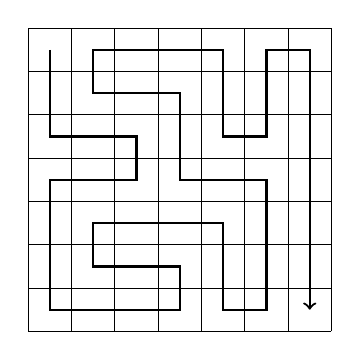
\begin{tikzpicture}[scale=.55]
  \begin{scope}
    \draw (0, 0) grid (7, 7);
    \draw[thick,->] (0.5,6.5) -- (0.5,4.5) -- (2.5,4.5) --
          (2.5,3.5) -- (0.5,3.5) -- (0.5,0.5) --
          (3.5,0.5) -- (3.5,1.5) -- (1.5,1.5) --
          (1.5,2.5) -- (4.5,2.5) -- (4.5,0.5) --
          (5.5,0.5) -- (5.5,3.5) -- (3.5,3.5) --
          (3.5,5.5) -- (1.5,5.5) -- (1.5,6.5) --
          (4.5,6.5) -- (4.5,4.5) -- (5.5,4.5) --
          (5.5,6.5) -- (6.5,6.5) -- (6.5,0.5);
  \end{scope}
\end{tikzpicture}
& \hspace{20px}
& 
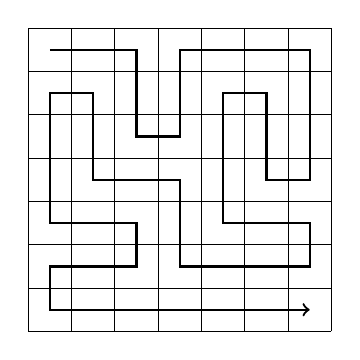
\begin{tikzpicture}[scale=.55]
  \begin{scope}[yscale=1,xscale=-1,rotate=-90]
    \draw (0, 0) grid (7, 7);
    \draw[thick,->] (0.5,6.5) -- (0.5,4.5) -- (2.5,4.5) --
          (2.5,3.5) -- (0.5,3.5) -- (0.5,0.5) --
          (3.5,0.5) -- (3.5,1.5) -- (1.5,1.5) --
          (1.5,2.5) -- (4.5,2.5) -- (4.5,0.5) --
          (5.5,0.5) -- (5.5,3.5) -- (3.5,3.5) --
          (3.5,5.5) -- (1.5,5.5) -- (1.5,6.5) --
          (4.5,6.5) -- (4.5,4.5) -- (5.5,4.5) --
          (5.5,6.5) -- (6.5,6.5) -- (6.5,0.5);
  \end{scope}
\end{tikzpicture}
\end{tabular}
\end{center}

بنابراین، می‌توان شرط کرد که گام اول همیشه به سمت پایین (یا راست) باشد و در پایان، تعداد پاسخ‌ها دو برابر شود.

\begin{itemize}
\item
زمان اجرا: ۲۴۴ ثانیه
\item
تعداد فراخوانی‌های بازگشتی: ۳۸ میلیارد
\end{itemize}

\subsubsection{بهینه‌سازی ۲}

اگر مسیر پیش از پیمایش تمام خانه‌های دیگر شبکه به خانهٔ پایین-راست برسد، واضح است که تکمیل پاسخ ناممکن خواهد بود. نمونه‌ای از این حالت مسیر زیر است:

\begin{center}
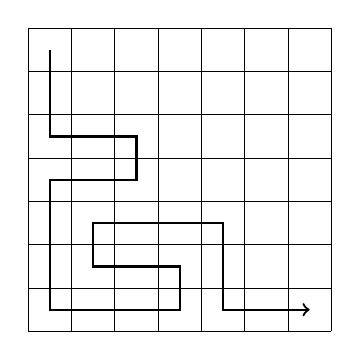
\begin{tikzpicture}[scale=.55]
  \begin{scope}
    \draw (0, 0) grid (7, 7);
    \draw[thick,->] (0.5,6.5) -- (0.5,4.5) -- (2.5,4.5) --
          (2.5,3.5) -- (0.5,3.5) -- (0.5,0.5) --
          (3.5,0.5) -- (3.5,1.5) -- (1.5,1.5) --
          (1.5,2.5) -- (4.5,2.5) -- (4.5,0.5) --
          (6.5,0.5);
  \end{scope}
\end{tikzpicture}
\end{center}
با تکیه بر این نکته، در صورت رسیدن زودهنگام به خانهٔ پایین-راست، جستجو را فوراً متوقف می‌کنیم.
\begin{itemize}
\item
زمان اجرا: ۱۱۹ ثانیه
\item
تعداد فراخوانی‌های بازگشتی: ۲۰ میلیارد
\end{itemize}

\subsubsection{بهینه‌سازی ۳}

اگر مسیر به دیوار برخورد کند و بتواند به چپ یا راست بپیچد، شبکه به دو بخش مجزا با خانه‌های دیده‌نشده تقسیم می‌شود. برای مثال، در وضعیت زیر مسیر می‌تواند به چپ یا راست برود:

\begin{center}
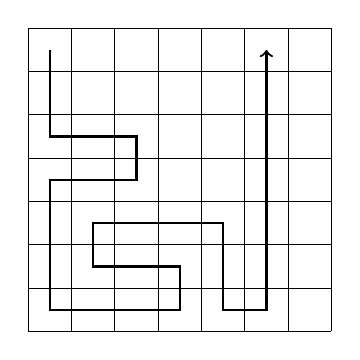
\begin{tikzpicture}[scale=.55]
  \begin{scope}
    \draw (0, 0) grid (7, 7);
    \draw[thick,->] (0.5,6.5) -- (0.5,4.5) -- (2.5,4.5) --
          (2.5,3.5) -- (0.5,3.5) -- (0.5,0.5) --
          (3.5,0.5) -- (3.5,1.5) -- (1.5,1.5) --
          (1.5,2.5) -- (4.5,2.5) -- (4.5,0.5) --
          (5.5,0.5) -- (5.5,6.5);
  \end{scope}
\end{tikzpicture}
\end{center}
در این حالت، پیمایش تمام خانه‌ها دیگر امکان‌پذیر نیست؛ پس جستجو متوقف می‌شود. این بهینه‌سازی بسیار کارآمد است:

\begin{itemize}
\item
زمان اجرا: ۱.۸ ثانیه
\item
تعداد فراخوانی‌های بازگشتی: ۲۲۱ میلیون
\end{itemize}

\subsubsection{بهینه‌سازی ۴}

ایدهٔ بهینه‌سازی ۳ را می‌توان تعمیم داد: اگر مسیر امکان حرکت رو به جلو نداشته باشد اما بتواند به چپ یا راست گردش کند، شبکه به دو بخش شامل خانه‌های دیده‌نشده تقسیم خواهد شد. برای مثال، مسیر زیر را ببینید:

\begin{center}
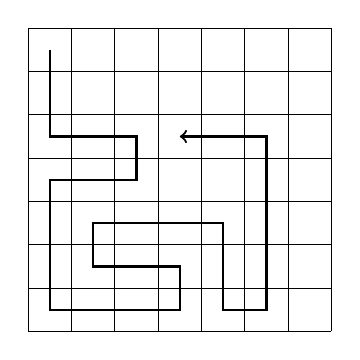
\begin{tikzpicture}[scale=.55]
  \begin{scope}
    \draw (0, 0) grid (7, 7);
    \draw[thick,->] (0.5,6.5) -- (0.5,4.5) -- (2.5,4.5) --
          (2.5,3.5) -- (0.5,3.5) -- (0.5,0.5) --
          (3.5,0.5) -- (3.5,1.5) -- (1.5,1.5) --
          (1.5,2.5) -- (4.5,2.5) -- (4.5,0.5) --
          (5.5,0.5) -- (5.5,4.5) -- (3.5,4.5);
  \end{scope}
\end{tikzpicture}
\end{center}
روشن است که دیگر نمی‌توان همهٔ خانه‌ها را پیمایش کرد؛ بنابراین جستجو قطع می‌شود. پس از این بهینه‌سازی، جستجو بسیار سریع عمل می‌کند:

\begin{itemize}
\item
زمان اجرا: ۰.۶ ثانیه
\item
تعداد فراخوانی‌های بازگشتی: ۶۹ میلیون
\end{itemize}

~\\
اکنون زمان مناسبی است تا بهینه‌سازی الگوریتم متوقف و نتایج بررسی شود. زمان اجرای الگوریتم اولیه ۴۸۳ ثانیه بود؛ حال با اعمال بهینه‌سازی‌ها، زمان اجرا به ۰.۶ ثانیه رسیده است. بنابراین الگوریتم نزدیک به ۱۰۰۰ برابر سریع‌تر شد.

این پدیده‌ای رایج در عقب‌گرد است،
زیرا درخت جستجو معمولاً بزرگ است
و حتی مشاهدات ساده نیز می‌توانند به شکلی مؤثر
جستجو را هرس کنند.
به‌ویژه بهینه‌سازی‌هایی که
در گام‌های اولیه الگوریتم رخ می‌دهند،
یعنی در بالای درخت جستجو، بسیار مفید هستند.

\section{ملاقات در میانه (Meet in the middle)}

\index{ملاقات در میانه}

\key{ملاقات در میانه} تکنیکی است
که در آن فضای جستجو به
دو بخش با اندازه‌های تقریباً برابر تقسیم می‌شود.
یک جستجوی جداگانه
برای هر دو بخش انجام می‌گیرد،
و در نهایت نتایج جستجوها با یکدیگر ترکیب می‌شوند.

از این تکنیک می‌توان استفاده کرد
اگر روشی کارآمد برای ترکیب
نتایج جستجوها وجود داشته باشد.
در چنین حالتی، این دو جستجو ممکن است زمان کمتری
نسبت به یک جستجوی بزرگ نیاز داشته باشند.
به‌طور معمول، با استفاده از تکنیک ملاقات در میانه
می‌توان ضریب $2^n$ را
به ضریب $2^{n/2}$ تبدیل کرد.

به‌عنوان مثال، مسئله‌ای را در نظر بگیرید که در آن
لیستی از $n$ عدد و
یک عدد $x$ داده شده است،
و می‌خواهیم بررسی کنیم آیا می‌توان
چند عدد از لیست را طوری انتخاب کرد که
مجموع آن‌ها برابر $x$ شود.
برای نمونه، با فرض لیست $[2,4,5,9]$ و $x=15$،
می‌توان اعداد $[2,4,9]$ را انتخاب کرد تا $2+4+9=15$ به دست آید.
با این حال، اگر برای همین لیست $x=10$ باشد،
تشکیل چنین مجموعی امکان‌پذیر نیست.

یک الگوریتم ساده برای این مسئله آن است که
تمام زیرمجموعه‌های عناصر را بررسی کنیم و
ببینیم آیا مجموع هر یک از زیرمجموعه‌ها برابر $x$ است یا خیر.
زمان اجرای چنین الگوریتمی $O(2^n)$ است،
زیرا $2^n$ زیرمجموعه وجود دارد.
اما با استفاده از تکنیک ملاقات در میانه،
می‌توان به الگوریتم کارآمدتری با زمان $O(2^{n/2})$ دست یافت\footnote{این
ایده در سال ۱۹۷۴ توسط E. Horowitz و S. Sahni معرفی شد \cite{hor74}.}.
توجه داشته باشید که $O(2^n)$ و $O(2^{n/2})$ پیچیدگی‌های متفاوتی
هستند، زیرا $2^{n/2}$ برابر با $\sqrt{2^n}$ است.

ایده کار تقسیم لیست به
دو لیست $A$ و $B$ است، به طوری که هر دو
لیست تقریباً نیمی از اعداد را در بر داشته باشند.
جستجوی اول تمام زیرمجموعه‌های
$A$ را تولید کرده و مجموع آن‌ها را در لیستی به نام $S_A$ ذخیره می‌کند.
به همین ترتیب، جستجوی دوم
لیست $S_B$ را از $B$ ایجاد می‌کند.
پس از این، کافی است بررسی شود که آیا می‌توان
یک عنصر از $S_A$ و عنصر دیگری
از $S_B$ انتخاب کرد به طوری که مجموع آن‌ها برابر $x$ شود.
این حالت دقیقاً زمانی ممکن است که راهی برای
تشکیل مجموع $x$ با استفاده از اعداد لیست اصلی وجود داشته باشد.

برای مثال، فرض کنید لیست $[2,4,5,9]$ و $x=15$ باشد.
ابتدا لیست را به $A=[2,4]$ و $B=[5,9]$ تقسیم می‌کنیم.
سپس، لیست‌های
$S_A=[0,2,4,6]$ و $S_B=[0,5,9,14]$ را می‌سازیم.
در این حالت، تشکیل مجموع $x=15$ امکان‌پذیر است،
زیرا $S_A$ شامل مجموع $6$ است،
$S_B$ شامل مجموع $9$ است، و $6+9=15$.
این متناظر با پاسخ $[2,4,9]$ است.

می‌توان الگوریتم را طوری پیاده‌سازی کرد که
پیچیدگی زمانی آن $O(2^{n/2})$ باشد.
ابتدا، لیست‌های \emph{مرتب‌شده} $S_A$ و $S_B$ را تولید می‌کنیم،
که با استفاده از تکنیکی شبیه به ادغام در زمان $O(2^{n/2})$ قابل انجام است.
پس از این، با توجه به مرتب بودن لیست‌ها،
می‌توان در زمان $O(2^{n/2})$ بررسی کرد که آیا
مجموع $x$ می‌تواند از $S_A$ و $S_B$ ساخته شود یا خیر.